%!TEX root = ../dokumentation.tex

\chapter{Beispiel Webframeworks}

\section{AngularJS}

\subsection{Allgemein}

\subsubsection{}


\subsubsection{Entwicklungsumgebung}
%% Hier besonders Angular Cli beschreiben


\subsection{Konzepte}
%% Beschreibung der Konzepte die in Angular verwendet werden
%% Hier kurz beschreiben wie die einzelnen Komponenten zusammenhängen

\begin{figure}
	\centering
	\label{fig:AngularAnwendung}
	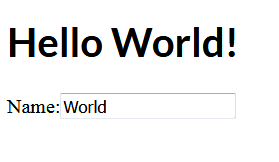
\includegraphics{angular-anwendung.png}
	\caption[Screenshot Angular-Beispielanwendung]{Screenshot Angular-Beispielanwendung} 
\end{figure}


Im Folgenden werden die in AngularJS verwendeten Konzepte näher erläutert. Die Beispielanwendung in \autoref{fig:AngularAnwendung} wird zur Erklärung der Konzepte verwendet. Bei Änderung des Namens im Input-Feld wird dieser in der obigen Überschrift auch verändert. Die Beispielanwendung weißt folgende Ordnerstruktur auf:

\begin{tabbing}
	mm \= mm \= mmmmmmmmmmmmmmmm \= \kill
	$\vdash$ \textbf{example/} \\ 
	| \> $\vdash$ \textbf{src/}\\ 
	| \> \> $\vdash$  \textbf{app/}\\
	| \> \>  --app.component.css  $\Rightarrow$ \textit{CSS-Datei von AppComponent}\\ 
	| \> \>  --app.component.html  $\Rightarrow$ \textit{Template von AppComponent}\\
	| \> \>  --app.component.ts	 $\Rightarrow$ \textit{Komponente AppComponent}\\
	| \> \>  --app.module.ts  $\Rightarrow$ \textit{Root-Modul AppModule}\\
	| \> \>  --hello.component.ts  $\Rightarrow$ \textit{Komponente HelloComponent}\\
	| \> \> $\vdash$ \textbf{assets/} \\
	| \> \> $\vdash$ \textbf{environments/} \\
	| \> --index.html\\
	| \> --main.ts\\
	| \> --styles.css \\
	| \> --... \\
	| \> $\vdash$ \textbf{node\_modules/}\\ 
	| \> $\vdash$ \textbf{e2e/}\\   
	| --...\\
\end{tabbing}

%% Erklärug am Beispiel des Initialen Projekts --> Mit Hinweis darauf, dass dies Projekt beliebig erweitert werden kann.
\subsubsection{Module}
Eine Angular Anwendung ist modular aufgebaut und kann demnach aus mehreren Modulen bestehen. Ein Modul fasst eine zusammengehörige Codeeinheit zusammen und kann eine gewisse Funktionalität bereitstellen, die wiederum von anderen Modulen verwendet werden kann. \autocites[vgl.][103\psqq]{Steyer.2017}  Die Module einer Angular-Anwendung können in Root-Module, Feature-Module und Shared-Module unterteilt werden. 

Jede Angular-Anwendung besitzt ein Root-Modul, das die Anwendung konfiguriert. Wenn ein Browser die Beispielseite anfordert, dann schickt der Server den Inhalt der \textit{index.html} als Antwort an den Browser zurück. Der Browser führt daraufhin die im HTML-Dokument enthaltenen Skript-Elemente aus. Dabei wird die Angular-Plattform initialisiert und das Root-Modul übergeben. \autocites[vgl.][60]{Steyer.2017}[vgl.][226\psqq]{Freeman.2018} In der Beispielanwendung stellt die Klasse \textit{AppModule} siehe \autoref{lst_RootModule} das Root-Modul dar. 

Module werden im Allgemeinen durch den Derokator \textit{@NgModule} gekennzeichnet und durch Eigenschaften konfiguriert. Ein Modul kann verschiedene weitere Module über die Eigenschaft \textit{import} importieren und damit die bereitgestellten Funktionalitäten verwenden. Die vom Modul verwendeten Direktiven, Komponenten und Pipes werden in der Eigenschaft \textit{declarations} angegeben. Jedes Root-Modul besitzt die Eigenschaft \textit{bootstrap}. Diese Eigenschaft spezifiziert die Komponente, die beim Starten der Anwendung geladen werden soll. 

Das Modul \textit{AppModule} in \autoref{lst:AppModule} importiert ein weiteres Modul mit dem Namen \textit{BrowserModule} und deklariert die zugehörige Komponente \textit{AppComponent}. Diese Komponente soll auch beim Start der Anwendung aufgerufen werden.

\begin{lstlisting}[caption=Das Root-Module in der Datei app.module.ts, label=lst:AppModule, language=Java]
import { NgModule } from '@angular/core';
import { BrowserModule } from '@angular/platform-browser';
import { FormsModule } from '@angular/forms';

import { AppComponent } from './app.component';
import { HelloComponent } from './hello.component';

@NgModule({
imports:      [ BrowserModule, FormsModule ],
declarations: [ AppComponent, HelloComponent ],
bootstrap:    [ AppComponent]
})
export class AppModule { }

\end{lstlisting}

Feature Modulen ermöglichen die Gruppierung einer Anwendung in Anwendungsfällen. Mithilfe von Shared-Module können die Teile einer Anwendung zusammengefasst werden, die unabhängig vom Anwendungsfall verwendet werden können. \autocites[vgl.][528\psqq]{Freeman.2018}[vgl.][]{Google.c}[vgl.][105\psqq]{Steyer.2017}

\subsubsection{Komponenten und Templates}

%Beschreibung des Starts einer Angular Anwedung 

%% Komponenten sind Direktiven 
%% Template und Komponente beschreiben
Komponenten sind Klassen, die Daten und Logik für die zugehörigen Templates bereitstellen. Diese ermöglichen die Aufteilung einer Angular Anwendung in logisch getrennte Teile. \autocite[vgl.][401]{Freeman.2018} 

Eine Komponente wird durch den Dekorator \textit{@Component} gekennzeichnet und kann über verschiedene Dekorator-Eigenschaften (auch: Metadaten) konfiguriert werden. Die Eigenschaft \textit{selector} identifiziert das HTML-Element, dass durch diese Komponente repräsentiert wird. Zur Anzeige der bereitgestellten Daten kann entweder ein Inline-Template \textit{template} definiert oder auf ein externes Template \textit{templateUrl} verwiesen werden. \autocites[vgl.][]{Google.b}[vgl.][405]{Freeman.2018}[vgl.][47\psqq]{Steyer.2017} 

Für weitere Dekorator-Eigenschaften wird auf \textcite[405]{Freeman.2018} verwiesen. Ein Beispiel für die Implementierung einer Komponente findet sich in \autoref{lst:AppComponentTs}.

\begin{lstlisting}[caption=Die Komponente AppComponent in der Datei app.component.ts, label=lst:AppComponentTs, language=Java]
import { Component } from '@angular/core';

@Component({
selector: 'my-app',
	templateUrl: './app.component.html',
	styleUrls: [ './app.component.css' ]
})
export class AppComponent  {
	name;
}
\end{lstlisting}

\begin{lstlisting}[caption=Die Komponente HelloComponent in der Datei hello.component.ts, label=lst:HelloComponentTs, language=Java]
import { Component, Input } from '@angular/core';

@Component({
	selector: 'hello',
	template: `<h1>Hello {{name}}!</h1>`,
	styles: [`h1 { font-family: Lato; }`]
})
export class HelloComponent  {
	@Input() name: string;
}
\end{lstlisting}


Zur Darstellung von Komponenten nutzt Angular Templates. Ein Template besteht aus HTML Code erweitert um Angular Ausdrücke. Das Template kann Pipes zur Formatierung von Daten, weitere Komponenten, Data-Binding Ausdrücke oder Direktiven enthalten. \autocites[vgl.][]{Google.b}[vgl.][52]{Steyer.2017} 

\begin{lstlisting}[caption=Das Template in der Datei app.component.html, label=lst:AppComponentHTML, language=HTML]
	<hello name="{{name}}"></hello>
	<label for="name">Name:</label>
	<input name="name" [(ngModel)]="name">
\end{lstlisting}

Data-Binding Ausdrücke stellen eine Beziehung zwischen den Daten der Komponente und einem HTML-Element her. Hierdurch kann das Aussehen, der Inhalt oder das Verhalten dieses Elements dynamisch verändert werden. In \autoref{tab:DataBinding} werden die Arten von Data-Bindings unterschieden. Die Unterscheidung erfolgt mittels der Fließrichtung der Daten. 

\begin{table}
\begin{tabular}{|>{\raggedright\arraybackslash}p{3cm}|>{\raggedright\arraybackslash}p{3.2cm}|>{\raggedright\arraybackslash}p{7cm}|}
	\hline
	\textbf{Richtung}&\textbf{Syntax}&\textbf{Verwendung}\\
	\hline 
	One-way Komponente -> View &\{\{Ausdruck\}\} \lbrack Ziel\rbrack =\dq Ausdruck\dq  & Interpolation, Eigenschaft, Attribut, Klasse, Style\\ 
	\hline 
	One-way Komponente <- View &(Ziel)=\dq Ausdruck\dq&Events\\ 
	\hline 
	Two-way&\lbrack (Ziel)\rbrack =\dq Ausdruck\dq&Formular\\ 
	\hline 
\end{tabular}
\caption{Arten von Data-Bindings}
\label{tab:DataBinding}
\end{table}

Das Ziel eines Data-Bindings ist entweder eine Attribut-Direktive oder eine Eigenschaft. Direktiven werden im nächsten Abschnitt näher erläutert. Der Ausdruck ist ein JavaScript-Fragement, der einen Zugriff auf die Eigenschaften und Methoden der Komponente ermöglicht. \autocites[vgl.][237\psqq]{Freeman.2018}[vgl.][52\psq]{Steyer.2017} [vgl.][]{Google.d} 


%%Verweis auf nächstes Kapitel

%% Wie funktioniert das einbinden einer weiteren Komponente? 
%% Was passiert beim Aufruf der Komponente???


\subsubsection{Direktiven}


%% Attribut und Struktur Direktive Beschreiben

Die im vorherigen Abschnitt beschriebenen Komponenten sind Direktiven mit einer eigenen View. Mit Direktiven kann einem Element zusätzliches Verhalten hinzugefügt werden. \autocite[vgl.][265]{Steyer.2017}[vgl.][401]{Freeman.2018} In Angular werden folgende drei Arten von Direktiven unterschieden. \autocite[vgl.]{Google.}

\begin{itemize}
	\item Komponenten
	\item Attribut-Direktiven
	\item strukturelle Direktiven 
\end{itemize}

Angular stellt Direktiven zur Verfügung (engl. Built-In Directives), die durch eigene Direktiven erweitert werden können. \autocite[vgl.][261]{Freeman.2018}

Mit strukturellen Direktiven kann der Inhalt des HTML-Dokuments angepasst werden, indem Elemente dem diesem hinzugefügt oder entnommen werden. Hierfür verwenden die strukturellen Direktiven Templates, die beliebig oft gerendert werden. \autocites[vgl.][269\psqq]{Steyer.2017}[vgl.][365]{Freeman.2018}

Beispiele für strukturellen Direktiven aus AngularJS \autocite[vgl.][261\psqq]{Freeman.2018}:
\begin{description}
	\item [ngIf] Fügt dem HTML-Dokument Inhalt hinzu, wenn die Bedingung wahr ist. 
	\item [ngfor] Fügt für jedes Item einer Datenquelle den gleichen Inhalt dem HTML-Dokument hinzu.
	\item [ngSwitch] Fügt dem HTML-Dokument, abhängig vom Wert eines Ausdrucks, Inhalt hinzu.
\end{description} 

Mit Attribut-Direktiven kann das Verhalten und Aussehen des zugehörigen Elementes angepasst werden, indem Attribute hinzugefügt oder entfernt werden. \autocite[vgl.][339]{Freeman.2018} 

Beispiele für Attribut-Direktiven aus Angular-JS \autocite[vgl.][249\psqq]{Freeman.2018}:
\begin{description}
	\item [ngStyle] Mit dieser Direktive können unterschiedliche Style-Eigenschaften dem Element hinzugefügt werden.
	\item [ngClass] Weißt dem Element ein oder mehrere Klassen hinzu. 
\end{description}

\subsubsection{Services}

%% Was bringen Services? Wie funktionieren diese?
%% Kommunkikation mit dem DB-Server über Services

%%\subsubsection{Pipes} 
%% ???


%%\subsubsection{Dependency Injection}
%% Was ermöglicht dieses Konzept? --> leichteres testen, lose Kopplung



\subsection{Verwendung}

\subsubsection{Einordnung in den Kontext}


\section{ReactJS}

\subsection{Allgemein}
%Entwicklung
%Kompatibilität
%Lizenz

%ReactJs ist kein MVC Framework! Welches Problem löst ReactJS?
% Kurz auf Flux eingehen????

ReactJS ist ein von Entwicklern des Unternehmens Facebook Inc. entwickeltes JavaScript Framework. \autoref{Gackenheimer.2015} 


%Löst bestimmte Probleme
%



\subsection{Konzepte}

\subsubsection{Components}

%Klasse und Methode
%Lifecycle einer Klasse
%Vorteile einer Klasse (State versus Props)

%Kurz auf JSX eingehen

\subsubsection{Lifecycle}

\subsubsection{Virtual DOM}

\subsection{Verwendung}




\section{OpenUI5}